\label{s:hz}
\subsection{Potentially Rocky Planets in the Habitable Zone}

\subsubsection{Selecting the Eta-Earth Sample}
Kepler is NASA's first mission capable of detecting Earth-size planets around Sun-like stars in one-year orbits.  One of its primary science goals is to determine the occurrence rate of potentially habitable, terrestrial-sized planets --- a value often referred to as eta-Earth.  Here we use the concept of a habitable zone to select a sample of planet candidates that are the right distance from their host stars and small enough to possibly have a rocky surface. A point that bears repeating is that no claims can be made regarding planetary habitability based on size and orbital distance alone \citep{Kane2012,Tasker2017}.   This sample is, however, of great value to the occurrence rate studies that enable planet yield estimates for various designs of future life-detection missions \citep{stark2015}. This eta-Earth sample is provided in Table~\ref{t:hz} and shown in Figure~\ref{f:hzPlot}.


Before applying thresholds on planet properties, we first select a sample based on disposition score (see \S\ref{s:scores}) in order to produce a sample of highly reliable planets orbiting G-type stars. At long orbital period and small radius, we are vulnerable to instrumental false alarms despite the significant improvements afforded us by the latest versions of metrics like Marshall, Skye, Rubble, Chases, and Model-shift. This is evident in the FGK dwarf sample of Figures~\ref{f:prCompleteness} and~\ref{f:prReliability} by comparing the relatively low reliability (51\% to 58\%) and completeness (74\% to 83\%) measurements in the bottom right boxes to others at shorter period and larger radius.  Removing candidates with score~$<$~0.5 results in a significant improvement in the sample reliability with a smaller degradation in the sample completeness (Figure~\ref{f:adjscore}).  The candidates reported in Table~\ref{t:hz} are $\approx$80\% reliable for the G-type stars and even higher for the K- and M-type stars. Note there is only one late F-type star in the sample.  Kepler was not designed to reach the habitable zones of F-type stars, nor did the target list include many such stars.
%There is a sharp transition in the distribution of scores at 0.5 for the false positive population (see Figure~\ref{s:).  [ I think this just made the discussion more confusing]


The DR25 catalog uses the transit depth and period, along with the DR25 stellar table of \citet{Mathur2017ApJS}, to derive the planet radius and the semi-major axis of the planet's orbit.  From these we calculate the insolation flux in units of the Earth's insolation flux,

\begin{equation}
S_{p} = \frac{R_{\star}^{2} \cdot (T_{\star}/5777)^{4}}{a^{2}} ,
\end{equation}

\noindent where $a$ is the semi-major axis of the planet's orbit in AU, \tstar{} is in Kelvin, 5777~K is the effective temperature of the Sun, R$_{\star}$ is the radius of the star, and thus \Splanet{} is in units relative to Earth. The errors for both insolation flux and radii include the errors from the DR25 stellar catalog. The habitable zone represents a range of orbits where the flux received by the host star allows for the possibility of surface liquid water on an Earth-size planet.  While the insolation limits for the habitable zone depends on the stellar temperature, it roughly falls from 0.2--1.7 $S_{\earth}$ (see Figure~\ref{f:hzPlot}). We use the empirical (recent Venus/early Mars) habitable zone of \citet{Kopparapu2013}.  To err on the side of inclusiveness, we include candidates whose one sigma error bars on the insolation flux overlap this empirical habitable zone.


\clearpage
%\LongTables

\begin{deluxetable*}{rrlrrrrrrr}
\tablecolumns{10}
\tabletypesize{\scriptsize}
\tablewidth{\linewidth}
\tablecaption{Habitable Zone Planet Candidates}
\tablehead{
\colhead{KOI} &
\colhead{KIC} &
\colhead{Kepler} &
\colhead{Period} &
\colhead{\rp} &
\colhead{\sp} &
\colhead{\tstar} &
\colhead{\rstar} &
\colhead{MES} &
\colhead{Score} \\ 
\colhead{} &
\colhead{} &
\colhead{} &
\colhead{[days]} &
\colhead{[\re]} &
\colhead{[\se]} &
\colhead{[K]} &
\colhead{[\rsun]} 
}
\startdata
172.02 & 8692861 & Kepler-69 c & 242.46130 & 1.73$^{+0.21}_{-0.22}$ & 1.59$^{+0.59}_{-0.45}$ & 5637$^{+113}_{-101}$ & 0.94$^{+0.12}_{-0.12}$ & 18.0 & 0.693 \\ 
238.03 & 7219825 & \nodata & 362.97828 & 1.96$^{+0.33}_{-0.29}$ & 1.81$^{+0.87}_{-0.60}$ & 6086$^{+133}_{-133}$ & 1.22$^{+0.20}_{-0.18}$ & 11.9 & 0.784 \\ 
438.02 & 12302530 & Kepler-155 c & 52.66153 & 1.87$^{+0.11}_{-0.12}$ & 1.28$^{+0.26}_{-0.25}$ & 3984$^{+71}_{-86}$ & 0.54$^{+0.03}_{-0.04}$ & 30.6 & 1.000 \\ 
463.01\tablenotemark{c} & 8845205 & Kepler-560 b & 18.47763 & 1.55$^{+0.32}_{-0.29}$ & 1.21$^{+0.72}_{-0.47}$ & 3395$^{+74}_{-67}$ & 0.28$^{+0.06}_{-0.05}$ & 78.0 & 0.001 \\ 
494.01 & 3966801 & Kepler-577 b & 25.69581 & 1.70$^{+0.21}_{-0.33}$ & 2.30$^{+1.17}_{-1.10}$ & 3787$^{+163}_{-204}$ & 0.48$^{+0.06}_{-0.09}$ & 35.9 & 1.000 \\ 
571.05\tablenotemark{a} & 8120608 & Kepler-186 f & 129.94410 & 1.18$^{+0.11}_{-0.14}$ & 0.23$^{+0.07}_{-0.06}$ & 3751$^{+75}_{-84}$ & 0.44$^{+0.04}_{-0.05}$ & 7.7 & 0.677 \\ 
701.03 & 9002278 & Kepler-62 e & 122.38740 & 1.72$^{+0.10}_{-0.07}$ & 1.24$^{+0.27}_{-0.19}$ & 4926$^{+98}_{-98}$ & 0.66$^{+0.04}_{-0.03}$ & 35.9 & 0.994 \\ 
701.04\tablenotemark{d} & 9002278 & Kepler-62 f & 267.29100 & 1.43$^{+0.08}_{-0.06}$ & 0.44$^{+0.09}_{-0.07}$ & 4926$^{+98}_{-98}$ & 0.66$^{+0.04}_{-0.03}$ & 14.3 & 0.000 \\ 
812.03 & 4139816 & Kepler-235 e & 46.18420 & 1.83$^{+0.12}_{-0.15}$ & 1.32$^{+0.29}_{-0.30}$ & 3950$^{+70}_{-86}$ & 0.49$^{+0.03}_{-0.04}$ & 18.0 & 1.000 \\ 
854.01 & 6435936 & Kepler-705 b & 56.05608 & 1.94$^{+0.12}_{-0.22}$ & 0.69$^{+0.15}_{-0.19}$ & 3593$^{+71}_{-86}$ & 0.49$^{+0.03}_{-0.06}$ & 19.3 & 0.996 \\ 
947.01 & 9710326 & Kepler-737 b & 28.59914 & 1.83$^{+0.16}_{-0.21}$ & 1.87$^{+0.52}_{-0.53}$ & 3755$^{+75}_{-84}$ & 0.46$^{+0.04}_{-0.05}$ & 45.7 & 1.000 \\ 
1078.03 & 10166274 & Kepler-267 d & 28.46465 & 1.87$^{+0.14}_{-0.22}$ & 1.95$^{+0.49}_{-0.55}$ & 3789$^{+75}_{-82}$ & 0.46$^{+0.04}_{-0.05}$ & 22.2 & 0.992 \\ 
1298.02\tablenotemark{d} & 10604335 & Kepler-283 c & 92.74958 & 1.87$^{+0.08}_{-0.10}$ & 0.78$^{+0.15}_{-0.14}$ & 4141$^{+83}_{-91}$ & 0.58$^{+0.03}_{-0.03}$ & 10.7 & 0.000 \\ 
1404.02 & 8874090 & \nodata & 18.90609 & 0.87$^{+0.16}_{-0.21}$ & 3.03$^{+2.29}_{-1.67}$ & 3751$^{+219}_{-219}$ & 0.45$^{+0.08}_{-0.11}$ & 10.1 & 0.955 \\ 
1422.02 & 11497958\tablenotemark{b} & Kepler-296 d & 19.85029 & 1.52$^{+0.19}_{-0.23}$ & 1.83$^{+0.68}_{-0.62}$ & 3526$^{+71}_{-78}$ & 0.38$^{+0.05}_{-0.06}$ & 25.1 & 1.000 \\ 
1422.04 & 11497958 & Kepler-296 f & 63.33627 & 1.18$^{+0.15}_{-0.18}$ & 0.39$^{+0.15}_{-0.13}$ & 3526$^{+71}_{-78}$ & 0.38$^{+0.05}_{-0.06}$ & 9.1 & 0.927 \\ 
1422.05 & 11497958 & Kepler-296 e & 34.14211 & 1.06$^{+0.13}_{-0.16}$ & 0.89$^{+0.33}_{-0.30}$ & 3526$^{+71}_{-78}$ & 0.38$^{+0.05}_{-0.06}$ & 10.5 & 0.984 \\ 
1596.02 & 10027323 & Kepler-309 c & 105.35823 & 1.87$^{+0.13}_{-0.17}$ & 0.41$^{+0.09}_{-0.10}$ & 3883$^{+69}_{-93}$ & 0.50$^{+0.04}_{-0.04}$ & 16.5 & 0.738 \\ 
2162.02 & 9205938 & \nodata & 199.66876 & 1.45$^{+0.18}_{-0.18}$ & 2.06$^{+0.76}_{-0.59}$ & 5678$^{+113}_{-102}$ & 0.92$^{+0.12}_{-0.12}$ & 11.1 & 0.920 \\ 
2418.01 & 10027247 & Kepler-1229 b & 86.82952 & 1.68$^{+0.12}_{-0.21}$ & 0.35$^{+0.08}_{-0.11}$ & 3576$^{+71}_{-85}$ & 0.46$^{+0.03}_{-0.06}$ & 11.7 & 0.937 \\ 
2626.01 & 11768142 & \nodata & 38.09707 & 1.58$^{+0.20}_{-0.21}$ & 0.81$^{+0.30}_{-0.25}$ & 3554$^{+71}_{-80}$ & 0.40$^{+0.05}_{-0.05}$ & 14.6 & 0.999 \\ 
2650.01 & 8890150 & Kepler-395 c & 34.98978 & 1.14$^{+0.07}_{-0.10}$ & 1.71$^{+0.35}_{-0.42}$ & 3765$^{+75}_{-83}$ & 0.52$^{+0.03}_{-0.05}$ & 10.1 & 0.985 \\ 
2719.02 & 5184911 & \nodata & 106.25976 & 1.50$^{+0.10}_{-0.16}$ & 1.99$^{+0.53}_{-0.58}$ & 4827$^{+129}_{-144}$ & 0.82$^{+0.06}_{-0.09}$ & 10.0 & 0.990 \\ 
3010.01 & 3642335 & Kepler-1410 b & 60.86610 & 1.39$^{+0.07}_{-0.10}$ & 0.84$^{+0.17}_{-0.16}$ & 3808$^{+69}_{-76}$ & 0.52$^{+0.03}_{-0.04}$ & 12.7 & 0.996 \\ 
3034.01 & 2973386 & \nodata & 31.02092 & 1.66$^{+0.12}_{-0.17}$ & 1.70$^{+0.40}_{-0.45}$ & 3720$^{+73}_{-81}$ & 0.48$^{+0.03}_{-0.05}$ & 11.9 & 1.000 \\ 
3138.01\tablenotemark{b} & 6444896 & Kepler-1649 b & 8.68909 & 0.49$^{+0.00}_{-0.00}$ & 0.47$^{+0.00}_{-0.00}$ & 2703$^{+0}_{-0}$ & 0.12$^{+0.00}_{-0.00}$ & 12.0 & 1.000 \\ 
3282.01 & 12066569 & Kepler-1455 b & 49.27684 & 1.75$^{+0.09}_{-0.13}$ & 1.28$^{+0.26}_{-0.26}$ & 3899$^{+78}_{-78}$ & 0.53$^{+0.03}_{-0.04}$ & 14.7 & 0.996 \\ 
3284.01 & 6497146 & Kepler-438 b & 35.23319 & 0.97$^{+0.06}_{-0.07}$ & 1.62$^{+0.37}_{-0.34}$ & 3749$^{+75}_{-84}$ & 0.52$^{+0.03}_{-0.04}$ & 11.9 & 1.000 \\ 
3497.01 & 8424002 & Kepler-1512 b & 20.35972 & 0.80$^{+0.12}_{-0.16}$ & 1.38$^{+0.58}_{-0.58}$ & 3419$^{+67}_{-76}$ & 0.34$^{+0.05}_{-0.07}$ & 19.6 & 1.000 \\ 
4005.01\tablenotemark{a} & 8142787 & Kepler-439 b & 178.13960 & 2.25$^{+0.22}_{-0.16}$ & 1.70$^{+0.47}_{-0.31}$ & 5431$^{+81}_{-81}$ & 0.88$^{+0.09}_{-0.06}$ & 17.8 & 0.997 \\ 
4036.01 & 11415243 & Kepler-1544 b & 168.81133 & 1.69$^{+0.10}_{-0.06}$ & 0.80$^{+0.17}_{-0.12}$ & 4798$^{+95}_{-95}$ & 0.71$^{+0.04}_{-0.03}$ & 14.8 & 0.965 \\ 
4087.01 & 6106282 & Kepler-440 b & 101.11141 & 1.61$^{+0.10}_{-0.08}$ & 0.65$^{+0.14}_{-0.11}$ & 4133$^{+74}_{-82}$ & 0.56$^{+0.03}_{-0.03}$ & 15.7 & 1.000 \\ 
4356.01\tablenotemark{a} & 8459663 & Kepler-1593 b & 174.51028 & 1.74$^{+0.14}_{-0.20}$ & 0.28$^{+0.09}_{-0.09}$ & 4367$^{+124}_{-155}$ & 0.45$^{+0.04}_{-0.05}$ & 11.0 & 0.976 \\ 
4427.01 & 4172805 & \nodata & 147.66173 & 1.59$^{+0.12}_{-0.14}$ & 0.23$^{+0.06}_{-0.05}$ & 3788$^{+76}_{-84}$ & 0.49$^{+0.04}_{-0.04}$ & 10.8 & 0.969 \\ 
4460.01 & 9947389 & \nodata & 284.72721 & 2.02$^{+0.30}_{-0.29}$ & 1.41$^{+0.55}_{-0.44}$ & 5497$^{+82}_{-74}$ & 1.08$^{+0.16}_{-0.16}$ & 10.7 & 0.972 \\ 
4550.01 & 5977470 & \nodata & 140.25194 & 1.84$^{+0.05}_{-0.12}$ & 1.28$^{+0.17}_{-0.24}$ & 4821$^{+76}_{-86}$ & 0.79$^{+0.02}_{-0.05}$ & 9.6 & 0.934 \\ 
4622.01 & 11284772 & Kepler-441 b & 207.24820 & 1.56$^{+0.09}_{-0.06}$ & 0.30$^{+0.06}_{-0.05}$ & 4339$^{+78}_{-87}$ & 0.55$^{+0.03}_{-0.02}$ & 9.7 & 0.975 \\ 
4742.01 & 4138008 & Kepler-442 b & 112.30530 & 1.30$^{+0.07}_{-0.05}$ & 0.79$^{+0.15}_{-0.11}$ & 4401$^{+78}_{-78}$ & 0.59$^{+0.03}_{-0.02}$ & 12.9 & 0.993 \\ 
7016.01 & 8311864 & Kepler-452 b & 384.84300 & 1.09$^{+0.20}_{-0.10}$ & 0.56$^{+0.32}_{-0.15}$ & 5579$^{+150}_{-150}$ & 0.80$^{+0.15}_{-0.07}$ & 7.6 & 0.771 \\ 
7223.01 & 9674320 & \nodata & 317.06242 & 1.59$^{+0.27}_{-0.12}$ & 0.54$^{+0.29}_{-0.13}$ & 5366$^{+160}_{-144}$ & 0.71$^{+0.12}_{-0.05}$ & 10.3 & 0.947 \\ 
7706.01 & 4762283 & \nodata & 42.04952 & 1.19$^{+0.08}_{-0.16}$ & 2.00$^{+0.55}_{-0.68}$ & 4281$^{+115}_{-140}$ & 0.48$^{+0.03}_{-0.06}$ & 7.5 & 0.837 \\ 
7711.01 & 4940203 & \nodata & 302.77982 & 1.31$^{+0.34}_{-0.12}$ & 0.87$^{+0.66}_{-0.22}$ & 5734$^{+154}_{-154}$ & 0.80$^{+0.21}_{-0.07}$ & 8.5 & 0.987 \\ 
7882.01 & 8364232 & \nodata & 65.41518 & 1.31$^{+0.08}_{-0.12}$ & 1.79$^{+0.49}_{-0.47}$ & 4348$^{+130}_{-130}$ & 0.65$^{+0.04}_{-0.06}$ & 7.2 & 0.529 \\ 
7894.01 & 8555967 & \nodata & 347.97611 & 1.62$^{+0.49}_{-0.15}$ & 0.97$^{+0.87}_{-0.27}$ & 5995$^{+163}_{-181}$ & 0.88$^{+0.27}_{-0.08}$ & 8.5 & 0.837 \\ 
7923.01 & 9084569 & \nodata & 395.13138 & 0.97$^{+0.12}_{-0.10}$ & 0.44$^{+0.20}_{-0.13}$ & 5060$^{+192}_{-174}$ & 0.87$^{+0.10}_{-0.09}$ & 10.0 & 0.750 \\ 
%7938.01 & 9469494 & \nodata & 275.56030 & 2.33$^{+0.53}_{-1.32}$ & 8.60$^{+6.29}_{-7.18}$ & 5989$^{+213}_{-192}$ & 2.47$^{+0.56}_{-1.40}$ & 7.5 & 0.508 \\ 
7954.01 & 9650762 & \nodata & 372.15035 & 1.74$^{+0.46}_{-0.14}$ & 0.69$^{+0.52}_{-0.18}$ & 5769$^{+155}_{-172}$ & 0.81$^{+0.21}_{-0.07}$ & 8.9 & 0.839 \\ 
8000.01 & 10331279 & \nodata & 225.48805 & 1.70$^{+0.43}_{-0.14}$ & 1.20$^{+0.90}_{-0.30}$ & 5663$^{+169}_{-152}$ & 0.78$^{+0.19}_{-0.07}$ & 8.7 & 0.975 \\ 
8012.01 & 10452252 & \nodata & 34.57372 & 0.42$^{+0.17}_{-0.12}$ & 0.37$^{+0.47}_{-0.19}$ & 3374$^{+112}_{-82}$ & 0.22$^{+0.09}_{-0.06}$ & 7.7 & 0.989 \\ 
8174.01 & 8873873 & \nodata & 295.06066 & 0.64$^{+0.07}_{-0.07}$ & 0.70$^{+0.28}_{-0.21}$ & 5332$^{+160}_{-144}$ & 0.76$^{+0.09}_{-0.09}$ & 7.4 & 0.665 \\ 
\enddata
\label{hzearthstab}
\tablenotetext{a}{Confirmed planet properties from NASA Exoplanet Archive on May 31, 2017 place object inside HZ.}
\tablenotetext{b}{Confirmed planet properties from NASA Exoplanet Archive on May 31, 2017 place object outside HZ.}
\tablenotetext{c}{Confirmed planet with vetting score less than 0.5.}
\tablenotetext{d}{Confirmed planet dispositioned as False Positive in DR25.}
\end{deluxetable*}



\begin{figure}[tb]
    \centering
    %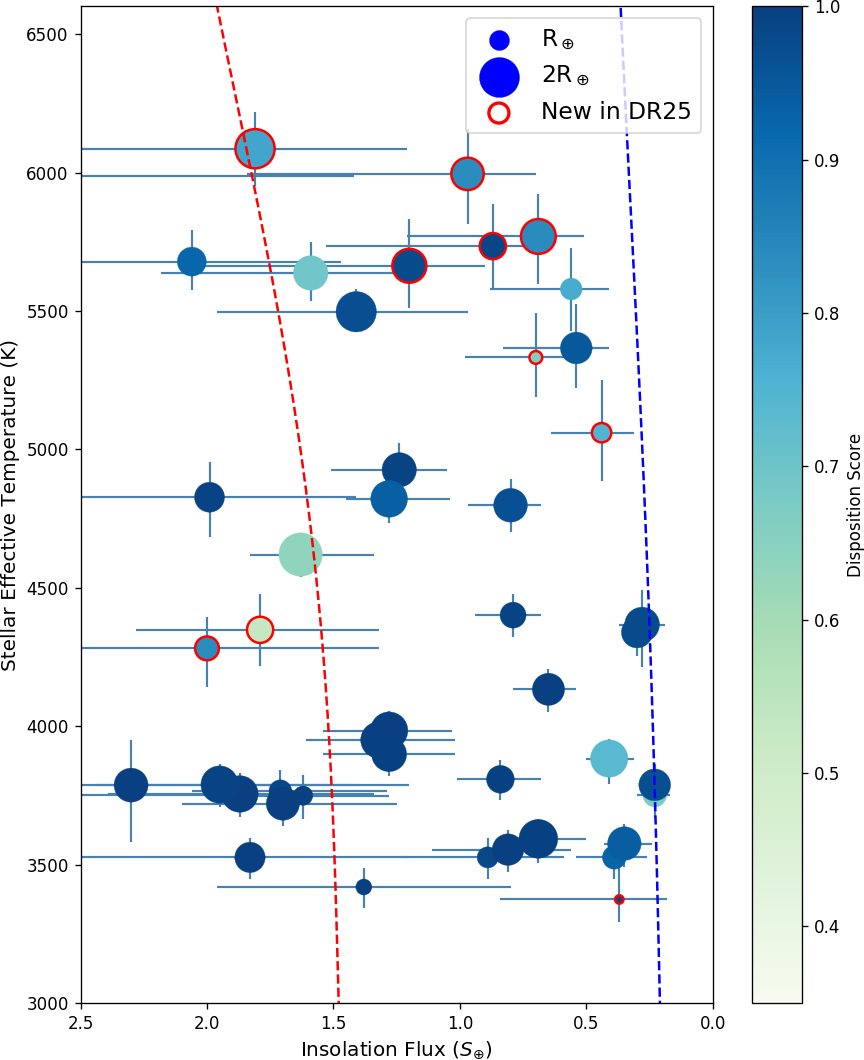
\includegraphics[width=\linewidth]{fig-hzTstarInsol-trimmed.png}
    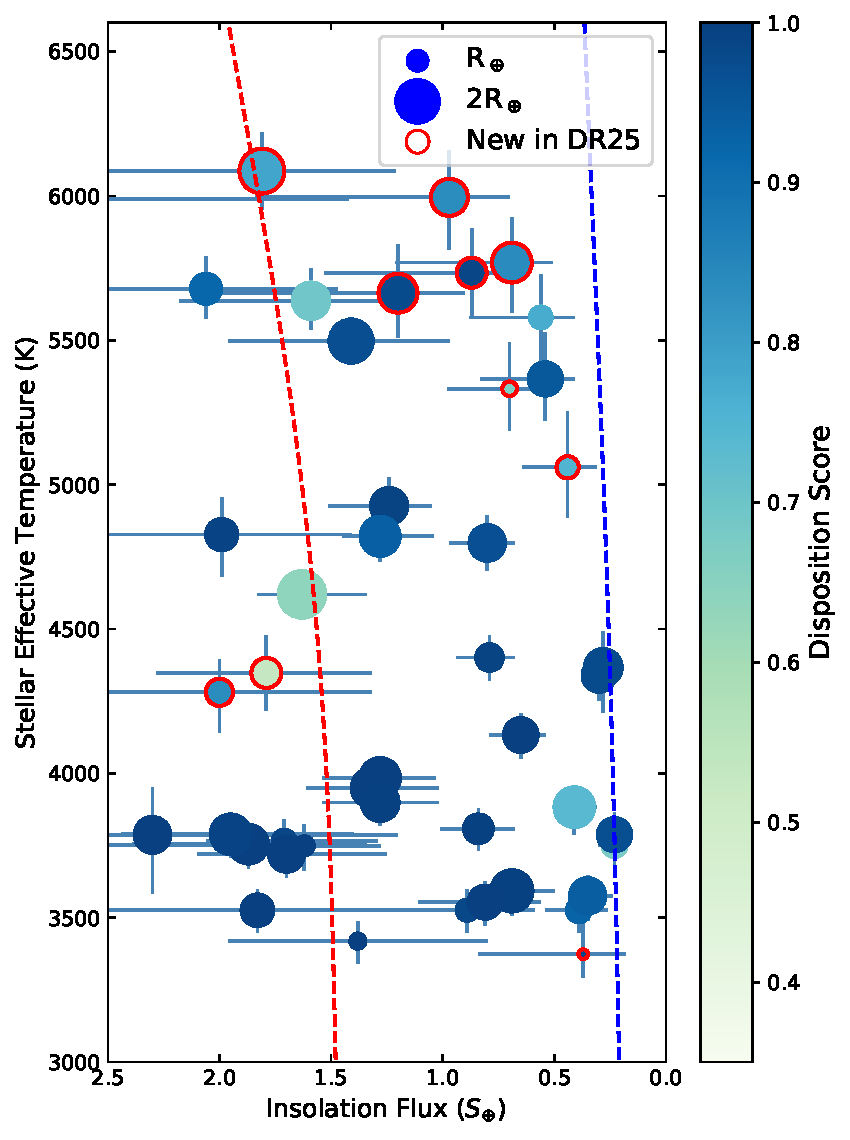
\includegraphics[width=\linewidth]{f14.pdf}
    \caption{DR25, eta-Earth sample of Planet Candidates plotted as stellar effective temperature against insolation flux using the values reported in the DR25 KOI catalog (which uses stellar properties from the DR25 stellar catalog \citep{Mathur2017ApJS}.) The size of the exoplanet is indicated by the size of the circle.  The color indicates the disposition score. Only those with disposition score greater than 0.5 are plotted.  Only objects whose error bars indicate that they could be in the habitable zone and have a radius less than 1.8~\re\ are shown. Those with a red ring are new to the DR25 catalog. }
    \label{f:hzPlot}
\end{figure}


Finally, we include only those candidates that satisfy the size constraint \rp~$- \sigma_{{R_p}\rm,low} < 1.8$~\re.  The purpose of the size constraint is to identify candidates likely to have a bulk composition similar to terrestrial planets in the solar system.  The 1.8~\re\ upper limit is taken from \citet{Fulton2017} who report a distinct gap in the radius distribution of exoplanets for planets in orbital periods of less than 100\,d.  The authors argue that the gap is the result of two (possibly overlapping) population distributions: the rocky terrestrials and the mini-Neptune size planets characterized by their volatile-rich envelopes.  Within this framework, the center of the gap marks a probabilistic boundary between having a higher likelihood of a terrestrial composition versus a higher likelihood of a volatile-rich envelope.  However, this boundary was identified using planets in orbital periods of less than 100\,days and it may not exist for planets in longer period orbits. Also it is not entirely clear that planets on the small side of this gap are all terrestrial. \citet{Rogers2015} examined small planets with density measurements with periods less than $\approx$50\,d and showed that less than half of planets with a radii of 1.62\,\re\ have densities consistent with a body primarily composed of iron and silicates.  For our purposes of highlighting the smallest planets in this catalog, we chose to be inclusive and set the threshold at 1.8\,\re.


To summarize, Table~\ref{t:hz} lists those candidates with scores greater than 0.5 and whose error bars indicate that they could be smaller than 1.8 \re{} and lie in the habitable zone. The table also includes KOI~2184.02 because the erratum to \citet{Mathur2017ApJS} (see \S\ref{s:stars} of this paper) reduces the stellar and planet radii so that the PC now lies in our sample. Note, the same erratum also reduces the planet radii of KOI~4460.01 and KOI~4550.01 to 2.0\,\re{} and 1.65\,\re{} respectively. The values reported in Table~\ref{t:hz} are identical to those in the KOI table at the NASA Exoplanet Archive and do not include the values reported in the erratum to \citet{Mathur2017ApJS}. Also, in order to make Table~\ref{t:hz} complete we include any \Kepler{} terrestrial-sized confirmed planet that falls in the habitable zone of its star according to the confirmed planet table at the Exoplanet Archive (downloaded on 2017-05-15). The objects are included, and denoted with footnotes, even if the DR25 catalog dispositions them as FPs, or if the DR25 planetary parameters place them outside the habitable zone. However, note that statistical inferences like occurrence rates should be based on a uniform sample drawn exclusively from the DR25 catalog and its self-consistent completeness and reliability measurements (see \S\ref{s:occurates}).  

%This is in section 8. Does it bare repeating?   
%We also note that future catalogs of updated star properties can have a significant impact on the eta-Earth sample and future missions will likely improve our understanding of the stellar properties and the planets they host. The catalog is designed to allow for updates to the stellar properties. 

We plot the eta-Earth sample candidates in Figure~\ref{f:hzPlot}, using only the information in the DR25 KOI catalog. Notice that this final search of the \Kepler{} data not only identified previously discovered candidates around the M dwarf stars, it also yielded a handful of highly reliable candidates around the GK dwarf stars. These GK dwarf candidates have fewer transits and shallower depths, making them much more difficult to find.  Despite their lower signal-to-noise, because we provide a measure of the reliability against false alarms (along with the completeness), these candidates are available to further study the occurrence rates of small planets in the habitable zone of GK dwarf stars.


\subsubsection{Notes on the Eta-Earth Sample}
Forty-seven candidates have a score greater than 0.5 and fall in this eta-Earth sample; 10 of these are new to this catalog (KOI numbers greater than 7621.01 and KOI~238.03).  A manual review of the 10 new high-score candidates indicates that they are all low signal-to-noise with very few transits, and show no obvious reason to be called false positives. However, our reliability measurements indicate that $\approx$20\% of these targets are not caused by a transiting/eclipsing system. As an example, the candidate most similar to the size and temperature of the Earth is KOI~7711.01 (KIC~004940203), with four transits that all cleanly pass the individual transit metrics. It orbits a 5734\,K star, has an insolation flux slightly less than that of Earth, and is about 30\% larger according to its DR25 catalog properties.  Plots showing visualizations of the transit data and its quality are available at the Exoplanet Archive for this object\footnote{\url{https://exoplanetarchive.ipac.caltech.edu/data/KeplerData/\allowbreak 004/004940/004940203/tcert/kplr004940203\_q1\_q17\_dr25\_obs\_tcert.pdf}} and for all of the \opstce{s}, \injtce{s}, \scrtce{s}, and \invtce{s}.


%\subsubsection{Notes on the Small Confirmed Planets in the Eta-Earth Sample}
Several confirmed planets fall in our eta-Earth sample.  Kepler-186f (KOI~571.05), Kepler-439b (KOI~4005.01) and Kepler-1593b (KOI~4356.01) move into the habitable zone according to the confirmed planet properties. They are included in Table~\ref{t:hz} with a footnote indicating they would not otherwise be listed. Kepler-296d (KOI~1422.02) and Kepler-1649b (KOI~3138.01), on the other hand, move outside the HZ according to the updated properties and are noted accordingly. Note, the default properties in the confirmed planets table at the Exoplanet Archive are selected for completeness and precision. Additional values may be available from other references that represent the best, current state of our knowledge.

Kepler-560b (KOI~463.01) is a confirmed planet that is a PC in the DR25 catalog, but failed the score cut; it is included for awareness and annotated accordingly.  The low score is caused by the Centroid Robovetter (\S\ref{s:centroidrv}) detecting a possible offset from the star's cataloged position, likely due to the star's high proper motion \citep{Mann2017}.  
%This target is assigned a minor flag (CENT_KIC_POS) alerting the user to the possibility of large errors in the source position from the Kepler Input Catalog.  A recent study (Mann et al 2017) yields …[TODO]

Two confirmed planets dispositioned as FPs in the DR25 catalog are included in Table~\ref{t:hz}: Kepler-62f (KOI~701.04) and Kepler-283c (KOI~1298.02).  Kepler-62f has only 4 transit events in the time series.  The transit observed during Quarter 9 is on the edge of a gap and narrowly fails Rubble.  The transit observed during Quarter 12 is flagged by the Skye metric.  Taken together, this leaves fewer than three unequivocal transits, the minimum required for the PC disposition. 

Kepler-283c (KOI~1298.02) fails the shape metric.  Its phase-folded transit appears v-shaped when transit timing variations are not included in the modeling.  We note that vetting metrics employed by the DR25 Robovetter were computed without consideration of transit timing variations, whereas the transit fits used in the KOI table, described in \S\ref{s:mcmc}, includes the timing variations as measured by \citet{Rowe2015cat}. 



\subsection{Caveats}
%{\color{blue}
When selecting candidates from the KOI catalog for further study, as we did for the eta-Earth sample (\S\ref{s:hz}), it is important to remember a few caveats. First, even with a high cut on disposition score, the reliability against false alarms is not 100\%. Some candidates may still be caused by false alarms, especially those around the larger, hotter stars. Also, this reliability number does not include the astrophysical reliability. Many of our tools to detect astrophysical false positives do not work for long-period, low MES candidates. For example, it is nearly impossible to detect the centroid offset created from a background eclipsing binary and secondary eclipses are not deep enough to detect for these stars. 

Second, the measured radius and semi-major axis of each planet depends on the stellar catalog.   As discussed in \S\ref{s:stars} and \citet{Mathur2017ApJS}, the stellar radii and masses are only known to a certain precision and the quality of the data used to derive these stellar properties varies between targets. These unknowns are reflected in the 1-sigma error bars shown in Figure~\ref{f:hzPlot} and listed in the KOI table. The uncertainty in the stellar information limits our knowledge of these planets.  As an example, for Kepler-452 (KIC~8311864), the DR25 stellar catalog lists a temperature of 5579$\pm150$\,K and stellar radius of 0.798$^{+0.150}_{-0.075}$\,\rsun, while the values in the confirmation paper \citep{Jenkins2015} after extensive follow-up are 5757$\pm85$\,K for the effective temperature and 1.11$^{+0.15}_{-0.09}$ for the stellar radius.  As a result, the planet Kepler-452b is given as 1.6$\pm0.2$\,\re\ in \citet{Jenkins2015} and 1.09$^{+0.2}_{-0.1}$\,\re\ in the DR25 catalog. The radii and stellar temperature differ by less than 2-sigma, but those differences change the interpretation of the planet from a super-Earth in the middle of the habitable zone of an early G dwarf host to an Earth-sized planet receiving about half the amount of flux from a late K star.  As follow-up observations of each candidate star is obtained and errors on the stellar parameters decrease, we expect this population to change in significant ways.  

Third, high-resolution imaging has proven crucial for identifying light from background and bound stars which add flux to the \Kepler{} photometric time series \citep{Furlan2017}. When this occurs, unaccounted for extra light dilutes the transit, causing the radii to be significantly underestimated \citep{Ciardi2015, Furlan2017densities}.  As a result, we fully expect that once follow-up observations are obtained for these stars, several of the PCs in this catalog, including those listed in the eta-Earth sample, will be found to have radii larger than reported in this catalog. 

%}


